\section{Compiler}\label{sec:compiler}
The purpose of a compiler is to convert source code into target code. In the case of the Arc compiler, the source code is text written in the Arc language. A generalized model of the compilation process can be seen in Figure~\ref{fig:generalcompilermodel}.

The target code is often low level code for a particular system or runtime, but not always. When the target code is another high level languange, the process is also called transpilation. The Arc languange is used for programming Arduinos, and so the compiler has to either generate Arduino specific machine code, or transpile to the high level Arduino language. Because the Arc language leverages the Protothreads library for the Arduino for its concurrency model, the Arc compiler is a transpiler.


\begin{figure}[htb!]
    \centering
    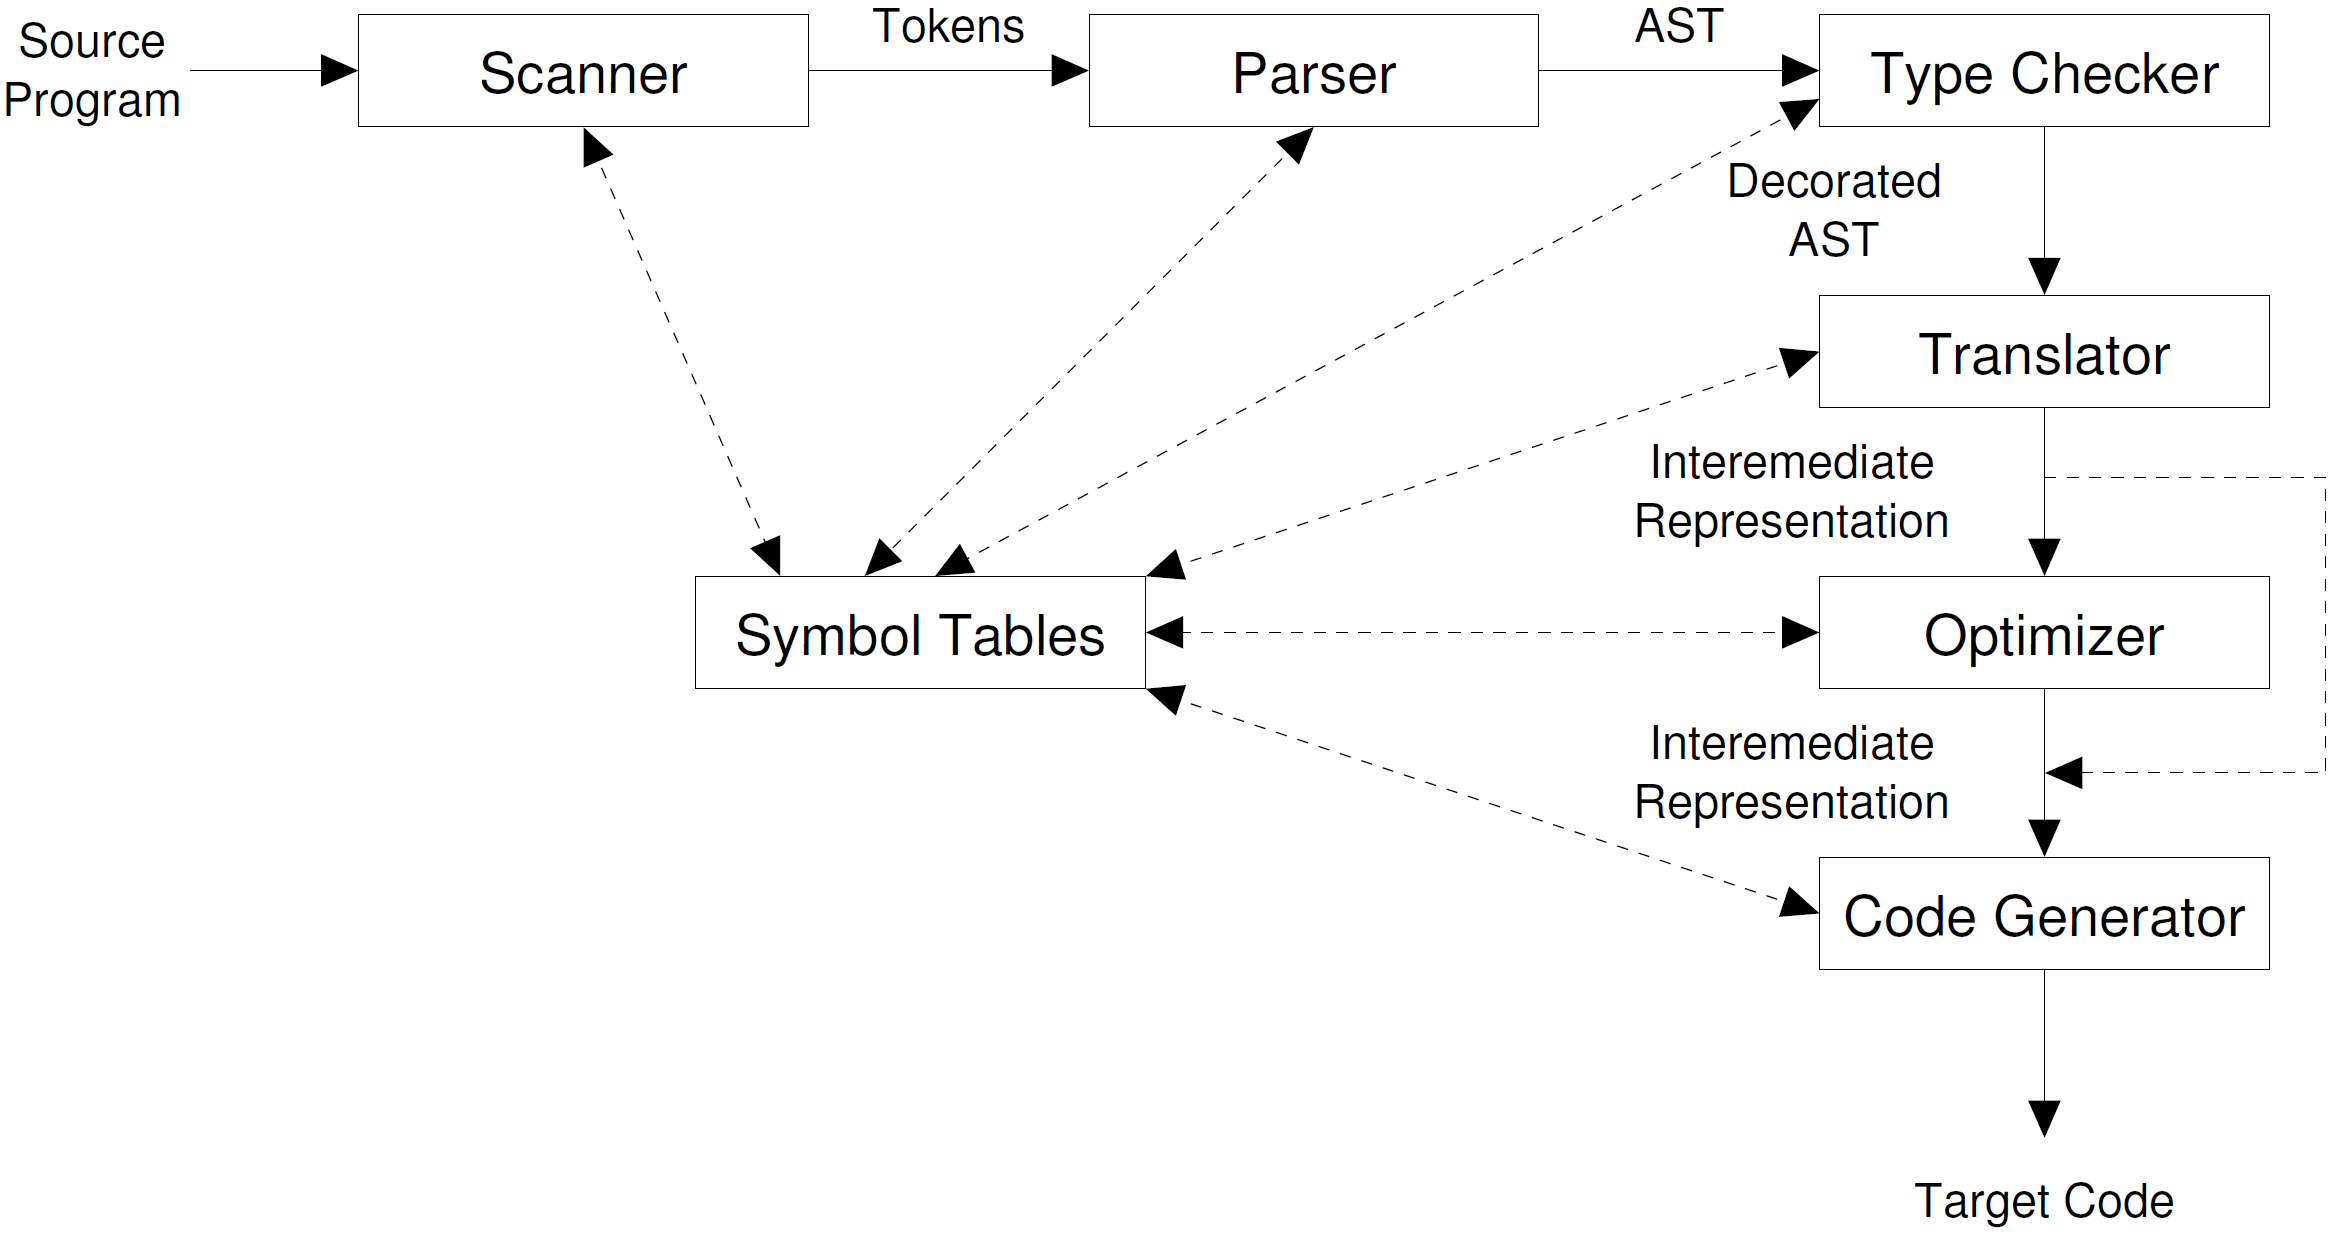
\includegraphics[width=0.8\textwidth]{figures/Full_Compiler.png}
    \caption{A general model of a compiler~\cite{CraftingCompiler}}
    \label{fig:generalcompilermodel}
\end{figure}


The Arc compiler follows many of the steps of the general model. Figure~\ref{fig:arccompilermodel} models the Arc compiler, with some noteworthy details.

\todo[inline]{Fill in the details of the model after image is added.}


\begin{figure}[htb!]
    \centering
    \missingfigure[figwidth=0.8\textwidth]{Insert image of the compilation process for the Arc transpiler}
    %\includegraphics[width=08\textwidth]{}
    \caption{The Arc compiler.}
    \label{fig:arccompilermodel}
\end{figure}


